\documentclass[../main.tex]{subfiles}

\begin{document}

\chapter[\hspace{0pt}绪\hskip\ccwd{}论]{{\heiti\zihao{3}\hspace{0pt}绪\hskip\ccwd{}论}}\label{chpt:1:intro}

本章内容共分为四节,\hyperref[section1: 研究背景及意义]{第一节}介绍本文的研究背景及意义;\hyperref[section1: 国内外研究现状与挑战]{第二节}总结少样本分类算法的国内外研究现状,并对其面临的挑战进行分析;\hyperref[section1: 本文研究内容与创新点]{第三节}介绍本文的研究内容与创新点;\hyperref[section1: 本文组织结构]{第四节}对本文组织结构进行概括。

\section[\hspace{-2pt}研究背景及意义]{{\heiti\zihao{-3} \hspace{-8pt}研究背景及意义}}\label{sec:1:reserach-background}

\subsection[\hspace{-2pt}深度学习技术的发展与演进]{{\heiti\zihao{4} \hspace{-8pt}深度学习技术的发展与演进}}\label{sec:1.1:deep-learning-evolution}

步入二十一世纪的第三个十年,以深度学习为核心驱动的人工智能技术,正以前所未有的广度与深度,对人类社会结构与科学研究范式产生着深远且结构性的影响。回顾深度学习的发展历程,可以清晰地观察到一条核心主线:对更高模型性能的追求,持续不断地推动着模型规模与复杂度的增长。

在深度学习发展的初期,以卷积神经网络(Convolutional Neural Networks, CNNs)和循环神经网络(Recurrent Neural Networks, RNNs)为代表的 “定制模型”(Bespoke Models)是主流。在这一阶段,模型结构需针对特定任务(如图像分类、语音识别)进行专门设计,并从随机初始化状态开始进行独立的端到端训练。AlexNet 等模型的成功证明了深度学习的巨大潜力,但这种模式的局限性也十分明显:一方面,模型知识难以在任务间复用,导致每一个新任务都意味着一次昂贵的、从零开始的研发循环;另一方面,模型性能高度依赖于大规模的标注数据,数据效率低下。尽管如此,为了在特定任务上取得更好的性能,研究者们已经开始通过加深网络层数、增加参数数量来提升模型的表达能力,模型规模的增长趋势已初现端倪。

为突破 “定制模型” 在知识复用和数据效率上的瓶颈,以迁移学习(Transfer Learning)思想为基础的 “预训练 - 微调”(Pre-training and Fine-tuning)方法应运而生,并迅速成为推动领域发展的主导力量。研究者发现,通过首先在 ImageNet 等大规模通用数据集上对模型进行预训练,可以使其学习到普适性的特征表示。其成功的理论基础在于深度神经网络的层级化特征学习机制:网络的浅层倾向于学习边缘、纹理等通用性底层特征,而深层则逐步组合这些特征,形成更抽象、更接近任务目标的语义概念。预训练过程正是为了捕获这种可复用的知识结构。随后,这个预训练好的模型可以作为 “基座”,通过在具体的下游任务上使用少量标注数据进行微调,即可快速获得优异的性能。这一变革极大地降低了对特定任务数据的依赖,显著提升了学习效率,成为深度学习应用普及的关键催化剂。更重要的是,它进一步强化并加速了模型规模的增长。为了获得更强大的通用特征表示,预训练模型的规模(包括深度、宽度和参数量)被不断推向新的高度,从数千万参数的 VGG 网络到上亿参数的 ResNet 系列,再到后来的 EfficientNet 等,模型规模的持续扩张与性能的提升形成了紧密的正相关关系。


\subsection[\hspace{-2pt}“规模驱动”范式下的效率困境]{{\heiti\zihao{4} \hspace{-8pt}“规模驱动”范式下的效率困境}}\label{sec:1.2:model-scale-growth}

近年来,在算力水平的指数级增长与数据资源的爆炸式累积双重驱动下,“预训练 - 微调” 范式最终演化为一种极致形态 —— 大规模预训练模型(Large-scale Pre-trained Models)的出现与确立。以基于 Transformer 架构的大语言模型(Large Language Models, LLM)和视觉基础模型(Vision Foundation Models)为代表,此类模型通过在万亿级别(Trillion-scale)的通用数据上进行自监督学习,将海量的世界知识(World Knowledge)与复杂的模式规律,隐式编码于其庞大的参数矩阵之中。其所展现的强大的零样本(Zero-shot)与少样本(Few-shot)泛化能力,以及在语言理解、逻辑推理、代码生成乃至跨模态交互等高级认知任务上达到的卓越性能,标志着人工智能领域已步入一个由 “基础模型”(Foundation Models)主导的新纪元。基础模型的 “基础” 性体现在,它们不再是面向单一任务的解决方案,而是作为一个通用的、可适配的智能基座,能够通过简单的提示(Prompting)或轻量化微调,支撑起一个庞大而多样化的应用生态。更值得注意的是,当模型规模突破某个阈值后,它们会表现出 “涌现能力”(Emergent Abilities),即在小模型上不存在、无法通过外推预测的能力,如上下文学习(In-context Learning)。此范式的成功不仅限于信息科学领域,更辐射至众多基础科学,例如 DeepMind 的 AlphaFold2 凭借深度学习技术对蛋白质结构预测这一生物学经典难题的突破,以及在材料科学、药物研发、高能物理等领域的应用,雄辩地证明了该技术路径的巨大潜力与普适价值。

然而,在由 “规模定律”(Scaling Law)—— 即模型性能随参数、数据和计算量的增加而可预测地提升 —— 所主导的技术路径之下,大规模模型所取得的巨大成功亦伴随着关于其可持续性与普适性的严峻挑战。其中,最为核心的制约因素集中体现在模型构建、训练与部署全周期内高昂的资源消耗,此可概括为 “效率困境”(Efficiency Dilemma)。该困境呈现为一种多维度、系统性的难题,正日益成为限制该领域健康发展的阿喀琉斯之踵。

其一,极为高昂的算力与经济成本所构筑的 “创新壁垒”。根据斯坦福大学发布的《2024 年人工智能指数报告》及相关研究,顶尖模型的训练成本正以超摩尔定律的速度攀升。例如,Google Gemini Ultra 模型的训练据估算需消耗高达 $5.0 \times 10^{25}$ FLOPs 的算力,其经济成本可达 1.91 亿美元。如此巨大的投入不仅在全球范围内形成了显著的 “算力鸿沟”,将绝大多数高校、研究机构与中小企业排斥在基础模型研发的门外,更可能引致创新活力的固化,将研究议程的设定权集中于少数科技巨头,甚至影响到国家间的科技竞争力。此外,高昂的算力消耗亦引发了对能源与环境影响的普遍关切。一次 GPT-3 级别模型的完整训练,其碳足迹可达数百吨二氧化碳当量,相当于一辆汽车绕地球行驶数十圈的排放量,这与全球对绿色计算和可持续发展的共识形成了鲜明对比。

其二,日益凸显的数据资源瓶颈与潜在的 “生态退化” 风险。大规模模型的性能高度依赖于海量、多样且高质量的训练数据。然而,据 Epoch AI 等研究机构的预测,若维持当前模型规模的增长速率,全球高质量的公开文本与图像数据可能在 2026 年至 2030 年间被消耗殆尽。数据资源的有限性构成了规模定律的根本物理约束。与此同时,生成式模型的广泛应用导致互联网正以前所未有的速度充斥着大量合成数据,这引致了对 “模型自噬”(Model Autophagy)或 “数据坍塌”(Data Collapse)现象的深切忧虑。该现象描述了一个恶性循环:模型在被自身或其他模型的输出所污染的数据集上进行迭代训练,可能导致知识的 “近亲繁殖”,即模型不断强化其自身的偏见与错误,而与真实世界逐渐脱节,最终引发性能衰退、多样性丧失与事实错误累积,从而威胁到整个数字知识生态的健康与发展。

其三,不容忽视的适配与部署成本所带来的 “应用鸿沟”。一个拥有数千亿参数的通用基础模型,即便已完成预训练,将其适配(Fine-tuning)至特定的下游任务,仍需可观的标注数据与计算资源。更关键的是,在众多对现实世界产生实际价值的应用场景中 —— 例如,需要植入智能手机的个人助手、要求实时决策的自动驾驶感知模块、或部署在物联网设备上的健康监测系统 —— 直接部署此类巨型模型在技术可行性与经济合理性上面临巨大障碍。这些障碍具体体现为:过大的内存占用(Memory Footprint),动辄数十 GB 的模型尺寸远超移动设备的 RAM 上限;无法接受的推理延迟(Inference Latency),复杂的计算使得单次推理耗时过长,无法满足实时交互的需求;以及高昂的能耗,持续运行大模型将迅速耗尽设备的电池电量。这使得大模型的强大能力难以 “下沉” 到资源受限的边缘端,形成了一条阻碍其普惠化的 “最后一公里” 鸿沟。

综上所述,尽管大规模深度学习模型已取得里程碑式的成就,但其对算力、数据、工程资源的极端依赖,已构成一个限制其应用广度、阻碍技术民主化、并引发可持续性质疑的根本性瓶颈。因此,探索深度模型的高效构建方法,实现从追求 “更大” 到注重 “更智” 的战略转向,已从一个单纯的技术优化选项,上升为决定深度学习技术能否健康、公平、可持续发展的核心科学议题。本研究即在此背景下展开,旨在为应对这一关键挑战提供系统性的算法与理论支持。

\section[\hspace{-2pt}核心科学问题]{{\heiti\zihao{-3} \hspace{-8pt}核心科学问题}}\label{sec:core-scientific-issues}

为系统性地应对上述宏观挑战,本论文将“效率”这一核心诉求,沿着从具体到抽象、从局部到全局的逻辑脉络,分解为三个层层递进的核心科学问题,共同构成了本研究的技术靶点。

\textbf{\circled{1} 单一场景下的高效知识继承}

在深度模型的应用生命周期中,最基础和最常见的需求是在一个明确定义的单一场景下实现效率优化。这通常表现为:给定一个或多个强大的、但因规模庞大而难以直接部署的预训练模型(教师模型),目标是为特定的下游任务构建一个轻量化、高效率的专用模型(学生模型)。例如,在智能手机上部署一个响应迅速的个人语音助手,或在车载芯片上运行一个低延迟的交通标志识别模型。这些应用场景对模型的内存占用、推理速度和能耗有着极为严苛的约束。

这一过程的核心挑战在于知识继承的保真度与效率之间的权衡。一方面,我们需要将教师模型中蕴含的丰富知识——不仅包括其最终的预测能力,更包括其对数据内在结构的理解、对语义关系的捕捉以及在高维特征空间中形成的几何流形,即所谓的“暗知识”(Dark Knowledge)——尽可能无损地迁移给学生模型。另一方面,这一迁移过程本身必须是高效的,尤其是在目标任务标注数据稀缺(即少样本学习)的条件下,如何避免学生模型在有限数据上过拟合,同时又能充分吸收教师模型的知识,成为一个非平凡的问题。传统的知识蒸馏方法在此类场景下可能效果不彰。因此,本论文的第一个核心科学问题是:如何在一个给定的、单一的应用场景中,设计出更优的知识迁移机制,以高效地继承已有模型的知识,从而在满足严格效率约束的同时,最大化专用模型的性能?

\textbf{\circled{2} 跨领域的普适知识迁移}

当面临一个全新的、不存在任何适用预训练模型的领域时,挑战一中以“知识继承”为前提的解决方案便不再适用。这类“冷启动”场景在科学计算(如基因组学、材料科学)、工业制造(如新型传感器数据分析)和新兴交叉学科中普遍存在。在这些领域,模型架构的设计往往是探索的第一步,也是最主要的瓶颈之一。传统上,架构设计高度依赖领域专家的经验和直觉,或诉诸于计算成本极其高昂的神经架构搜索(NAS),后者需要对成千上万个候选架构进行完整的训练和评估。

此时,挑战从迁移具体的“模型知识”升级为迁移更为抽象的“架构知识”。其核心假设是,尽管不同领域的任务和数据形态迥异,但构成高性能神经网络的底层设计原则(如有效的特征提取模块、促进梯度流动的连接方式、平衡深度与宽度的策略等)可能具有跨领域的普生性。然而,这些原则通常是隐式的,且不同架构搜索空间(Search Spaces)的定义方式(即编码方式)千差万别,这为知识的直接迁移带来了巨大障碍。因此,本论文的第二个核心科学问题是:如何定义并学习一种通用的、可跨越不同领域和异构搜索空间的架构知识表示,并利用这种表示来指导新领域下的架构搜索,从而实现模型设计过程的冷启动加速?

\textbf{\circled{3} 多源模型能力的系统性融合}

随着AI应用的深化,一个组织或研究者通过解决前两类问题,往往会积累一批针对不同任务的、能力各异的“专家模型”。例如,一个企业可能同时拥有一个用于代码生成的模型、一个用于合同审查的模型和一个用于市场分析的模型。这些模型各自在其专业领域内表现卓越,但它们的能力是分散和孤立的,形成了所谓的“模型孤岛”(Model Silos)。若要构建一个能够处理复合型任务(例如,“根据市场分析报告,起草一份包含代码示例的软件开发合同”)的通用模型,传统方法(如在一个超大模型上对所有任务进行联合训练)将面临灾难性的计算成本和数据整合难题。

此时,挑战演变为如何对这些已有的、分散的专家能力进行系统性的整合与升华。这不仅是简单的能力叠加,更追求实现“1+1 > N”的超加性效应,即融合后的模型在处理单一任务时性能不减,同时在处理多任务或新任务时展现出更强的泛化能力。这一过程的难点在于,模型的能力固化在其高度非线性的参数空间中,简单的参数平均或拼接往往会导致灾难性遗忘或能力冲突。因此,本论文的第三个核心科学问题是:如何设计一种高效且可扩展的机制,以系统性地融合来自多个独立专家模型的能力,从而在避免高昂再训练成本的同时,构建一个能力更全面、更强大的统一模型?

这三个挑战从单一场景的知识继承,到跨领域的知识迁移,再到多源能力的系统性融合,构成了一个逻辑严谨、层层递进的研究框架,旨在从根本上探索深度模型高效构建的通用原理。

\section[\hspace{-2pt}核心论点与研究思路]{{\heiti\zihao{-3} \hspace{-8pt}核心论点与研究思路}}\label{sec:core-idea}

面对上述三个看似不同但内在关联的挑战,本论文旨在论证一项统一的核心论点:将知识迁移(Knowledge Transfer)作为基本原则与核心机制,是实现深度模型高效构建的关键技术路径。

在机器学习领域,知识迁移广义上指将一个或多个源任务中获得的知识,应用于一个不同但相关的目标任务的过程。这一思想与人类的学习模式高度一致:我们并非孤立地学习每一项新技能,而是不断地利用已有知识来加速新知识的获取。与之形成鲜明对比的是,传统的模型构建范式,无论是从随机初始化开始训练,抑或在单一预训练模型上进行微调,其本质仍可归为“孤立学习”(Isolated Learning)。该范式隐含地假定各任务的学习过程相互独立,从而导致了知识资产的巨大浪费:在训练新模型时,未能充分利用其他相关模型已习得的知识;在设计新架构时,未能借鉴其他领域已验证的成功设计模式;在集成多源能力时,缺乏有效的知识融合范式。我们认为,当前模型构建的效率瓶颈,其根源即在于这种知识的“一次性使用”和“孤岛化”存储。

知识迁移,作为一个更广义的理论框架,其核心要义在于打破学习过程的孤立状态,承认并利用不同模型、任务、领域之间存在的内在关联性。通过将一个或多个源域(Source Domain)中获取的知识,以系统化的形式迁移并应用于目标域(Target Domain),能够显著加速学习过程、降低对数据与算力的依赖,并提升最终模型的性能与泛化能力。

基于此核心论点,本论文的研究思路是围绕知识的“表示、迁移、融合”这一主线,探索在不同抽象层次上实施知识迁移的机制与算法。具体而言,本论文的研究工作将沿循一条从具体到抽象、从微观到宏观的路径,对前述三个挑战逐一进行攻关,每一层次的研究都为解决相应挑战提供了理论与实践基础:

\textbf{\circled{1} 模型内部知识的迁移。} 为回应第一个挑战,本研究将知识界定为蕴含于大型“教师”模型参数矩阵中的、细粒度的隐式表征。这是知识最直接的载体。研究重点在于设计更为高效的知识蒸馏算法,以期将这些参数化知识近乎无损地迁移至一个轻量化的“学生”模型中。此为在最基础的粒度上对知识进行利用,旨在解决特定应用场景下的模型高效定制问题。

\textbf{\circled{2} 模型架构知识的迁移。} 为回应第二个挑战,本研究将知识的抽象层次提升至模型结构本身,将其界定为关于“何为优良计算图”的、可泛化的设计原则与模式。这种知识不再是具体的参数值,而是关于如何组织计算流的“蓝图”。研究重点在于探索如何从众多已有模型中萃取此类“元知识”(Meta-knowledge),并将其迁移至一个全新的领域,用以高效指导神经架构搜索。

\textbf{\circled{3} 模型任务能力的迁移与融合。} 为回应第三个挑战,本研究在最高的抽象层次上展开,将知识界定为模型作为一个功能整体所涌现出的、解决特定任务的“功能性能力”(Functional Capability)。这种知识是模型行为层面的体现。研究重点在于探索如何将此种能力从模型的复杂参数中解耦,进行独立的表示、操控与组合,从而实现一种“能力代数”,以达成多源能力的系统性融合。

通过对这三个层次知识迁移的系统性研究,本文旨在构建一个覆盖模型构建主要环节的高效算法体系。此三项工作并非相互孤立,而是共享同一哲学思想、互为支撑的有机整体,共同为“知识迁移是实现深度模型高效构建的关键路径”这一核心论点,提供了来自不同维度、层层递进的坚实论据,形成了一个完整而自洽的理论与实践框架。

\section[\hspace{-2pt}本文研究内容与主要贡献]{{\heiti\zihao{-3} \hspace{-8pt}本文研究内容与主要贡献}}\label{sec:research-content-and-contribution}

本论文在“知识迁移”这一核心思想的指引下,针对前述三个具体挑战,开展了系统性的算法研究与实验验证。主要的研究工作和创新贡献可具体归纳如下,每一项贡献都直接回应了前述的一个核心挑战:

\begin{enumerate}
	\item 针对模型知识迁移,提出了 Prompt-Distiller,一种面向提示式语言模型的少样本知识蒸馏框架。 该工作聚焦于如何将大型教师语言模型的知识高效迁移至小样本场景下的轻量化学生模型。我们识别出传统知识蒸馏方法在提示学习(Prompt-based Learning)范式下面临的挑战,并提出了一种双重对比学习(Dual Contrastive Learning)机制。该机制一方面在样本级别进行对比,促使学生模型学习教师模型对不同样本的区分能力;另一方面在标签级别进行对比,促使学生模型理解不同任务标签间的语义关系。通过这种方式,Prompt-Distiller 能够更全面、更鲁棒地迁移教师模型中的隐式知识,在多个少样本分类任务上的实验证明,该方法显著优于现有的知识蒸馏基线,为在资源受限场景下高效定制专用语言模型提供了有效途径。
	\item 针对架构知识迁移,提出了基于表征学习的演化式跨空间迁移神经架构搜索方法。 为解决新领域架构设计的冷启动难题,该工作旨在实现架构知识在不同搜索空间(Search Spaces)之间的有效迁移。我们提出了一种创新的演化迁移神经架构搜索(Evolutionary Transfer NAS)框架。其核心是学习一种通用的架构表征(Representation),该表征能够将不同搜索空间中的架构映射到一个统一的潜在空间中。在此基础上,通过演化算法在该潜在空间中进行搜索,并将从源领域搜索过程中学到的知识(如优秀的架构基因片段)迁移至目标领域的搜索任务中。这种基于表征学习的迁移机制,使得算法能够跨越不同架构编码方式的鸿沟,显著加速在新领域中发现高性能架构的过程,有效降低了 NAS 的应用成本。
	\item 针对任务能力融合,提出了 MFTO,一种基于多形式迁移优化的多任务模型高效融合框架。该工作旨在解决大规模多任务学习场景下,如何高效融合多个监督微调(SFT)后的专家模型的问题。面对融合配方搜索的组合爆炸与非凸优化难题,我们提出了多形式迁移优化(Multi-Form Transfer Optimization, MFTO)方法。其核心思想是 “分而治之,迁移学习”:首先,将复杂的大规模融合问题智能地分解为多个小规模、多样化的子问题(即多样的 “形式”,Forms);其次,并行地在这些子问题上使用优化器进行探索,以低成本收集关于模型 - 任务关系的局部经验,如任务间的协同 / 冲突关系矩阵、参数在不同任务中的重要性等;最后,将这些宝贵的局部经验作为高质量的先验知识,迁移回原始的全局优化问题中,从而指导全局优化器在巨大的搜索空间中进行高效探索,快速定位近似最优的融合配方。该框架通过局部经验积累与全局指导相结合,为解决大规模模型融合这一以往依赖启发式或面临计算瓶颈的难题,提供了一种系统性的、可扩展的优化范式,为实现“1+1 > N”的超加性能力集成铺平了道路。
\end{enumerate}

\section[\hspace{-2pt}本文结构安排与符号约定]{{\heiti\zihao{-3} \hspace{-8pt}本文结构安排与符号约定}}\label{sec:structure-and-symbols}

本文共分为六章,其组织结构如下:

第一章:绪论。 本章阐述了研究工作的宏观背景与现实动机,系统分析了当前大规模模型范式下的效率困境,并在此基础上清晰地界定了本文旨在解决的三个层层递进的科学问题。随后,提出了贯穿全文的核心论点 —— 以知识迁移作为高效构建模型的根本路径,并阐述了在模型知识、架构知识和任务能力三个层次上的具体研究思路,最后概述了本文的主要创新贡献。

第二章:相关工作。 本章将对与本研究密切相关的理论基础和技术现状进行系统性的回顾与评述。内容将主要围绕三个核心领域展开:知识蒸馏(Knowledge Distillation)的各类方法,特别是面向提示学习的方法;可迁移神经架构搜索(Transferable NAS),重点关注跨领域和跨搜索空间的技术;以及模型融合(Model Merging),包括基于参数平均、任务算术和优化搜索的各类方法。

第三章:面向提示学习的少样本知识蒸馏。 本章将详细介绍为解决第一个挑战而设计的 Prompt-Distiller 框架。内容将包括其核心理论 —— 双重对比学习机制,具体的算法设计与实现细节,以及在一系列少样本自然语言理解任务上的详尽实验结果与深入分析,以证明其有效性。

第四章:基于表征学习的跨空间演化迁移神经架构搜索。 本章将详细阐述为解决第二个挑战而设计的演化迁移 NAS 方法。将重点介绍其统一的架构表征学习模块(基于 VAE 和 Transformer)、跨空间映射机制,以及演化序列迁移优化算法。最后,通过在 NAS-Bench-101、NAS-Bench-201 和 DARTS 等多个异构搜索空间上的实验,验证该方法的有效性和高效率。

第五章:基于多形式迁移优化的多任务模型融合。 本章将聚焦于第三个挑战,详细介绍所提出的 MFTO 框架。内容将涵盖问题分解策略、局部经验(如任务协同 / 冲突矩阵)的获取方法,以及如何将这些经验迁移以指导全局融合配方搜索的完整流程。此外,将通过在大规模多任务场景下的实验,展示该方法在提升融合效率与性能方面的强大效果。

第六章:总结与展望。 本章将对全文的研究工作进行全面、系统的总结,重申本文的核心发现与贡献,并讨论其理论意义与实践价值。在此基础上,将探讨当前工作的潜在局限性,并对未来可能的研究方向进行展望,例如将三种知识迁移方法进行更深度的结合,形成一个统一的、自动化的模型构建流水线,以及探索该理论框架在多模态、多智能体等更复杂场景下的应用潜力。

\end{document}

% \section[\hspace{-2pt}研究背景及意义]{{\heiti\zihao{-3} \hspace{-8pt}研究背景及意义}}\label{section1: 研究背景及意义}

% \section[\hspace{-2pt}国内外研究现状与挑战]{{\heiti\zihao{-3} \hspace{-8pt}国内外研究现状与挑战}}\label{section1: 国内外研究现状与挑战}

% \subsection[\hspace{-2pt}研究现状]{{\heiti\zihao{4} \hspace{-8pt}研究现状}}\label{section1: 研究现状}

% 近年来,已有很多少样本分类方法被提出,按其技术方案可以大致分为五类,分别是:基于元学习的少样本算法、基于度量的少样本算法、基于数据增强的少样本算法、基于特征学习的少样本算法和基于语义的少样本算法,以下将分别对其进行介绍。

% \textbf{(1)基于元学习的少样本算法}

% 基于元学习的少样本分类算法\cite{MAML, lee2019meta, LEO, 元学习},其核心思想是在训练阶段便模拟少样本测试任务,在从基类数据集采样的大量少样本分类任务中学习到元知识,元知识可以迁移到其他少样本任务,从而使模型在遇到新任务时能够通过极少量的样本训练便快速调整参数并达到较好的分类性能。例如,Finn等人\cite{MAML}提出了模型无关的元学习算法(Model-Agnostic Meta-Learning,简称 MAML)。MAML设计了一种优化算法,通过找到一组初始化模型参数,使用少量梯度下降便能够使其适应新的任务。Lee等人\cite{lee2019meta}则是使用支持向量机(Support Vector Machine,简称SVM)代替MAML方法中的线性分类器,并结合了一个可微分二次规划求解器使得其能够端到端学习。Rusu等人\cite{LEO}提出了一种在低维潜在空间进行模型元学习的方法LEO,其将元学习问题转化为潜在空间中的优化问题,利用潜在空间的特征嵌入捕捉少样本任务间共享的结构性知识,促进不同任务间的知识转移。基于元学习的方法虽很符合少样本分类的特点,但其通常需要先对特征提取网络进行预训练,并在元学习阶段采样大量任务来微调网络,存在训练过程较为复杂的问题。

% \textbf{(2)基于度量的少样本算法}

% 基于度量的方法\cite{ProtoNet, vinyals2016matching, DeepEMD, 度量学习}为少样本分类问题提供了另一种解决思路,其旨在通过学习样本之间的距离或相似度度量来处理少样本问题。这类方法的核心思想是,如果能够合理地度量样本之间的距离或相似性,即便是只有少量的训练样本,也可以通过比较未知样本与已知样本之间的距离或相似度来进行有效的分类。基于度量的方法大多使用欧式距离、余弦相似度计算样本之间的距离,例如Snell等人\cite{ProtoNet}提出的原型网络(Prototypical Networks, 简称ProtoNet)。ProtoNet基于以下假设:在特征空间中,每个类别都可以由其样本特征的平均值代表的一个原型来表示。在进行分类时,其会计算查询样本与每个类别原型之间的欧式距离,并将查询样本分类到最近的原型所代表的类别。Zhang等人\cite{DeepEMD}提出的DeepEMD方法为少样本分类引入了一种新的距离度量方式:推土机距离(Earth Mover's Distance,简称EMD)。DeepEMD将一张图像分为不同的图像块,对其进行特征提取并利用推土机距离作为度量标准来比较不同图像之间的相似度。另外,Sung等人\cite{RelationNet}提出的关系网络(Relation Networks,简称RelationNet)则是通过学习一个深度度量来评估样本之间的关系得分,进而通过关系得分进行分类。与之前方法不同,此关系得分是通过网络学习到的,而不是设计的固定距离度量方式。基于度量的少样本算法简单高效,其难点主要在于如何建立一个合适的度量方式来衡量样本之间的距离或相似度。

% \textbf{(3)基于数据增强的少样本算法}

% 增加样本数量来应对标注样本不足的问题,是少样本分类最直观的解决方案,因此,基于数据增强的少样本算法被提出\cite{IDeMe-Net, AFHN}。少样本分类中,每个类别样本数目极少,模型很容易产生过拟合问题,该类算法通过增加训练样本的数量和多样性来帮助模型学习到更加鲁棒的特征表示,从而减少过拟合的风险。例如,Chen等人\cite{IDeMe-Net}提出了一种名为图像变形元网络(Image Deformation Meta-Networks,简称IDeMe-Net)的新颖框架。IDeMe-Net训练一个网络,该网络能够通过线性地融合一组图像生成变形图像,从而产生额外的标注样本,增加模型的训练样本。Li等人\cite{AFHN}提出的对抗性特征幻觉网络(Adversarial Feature Hallucination Networks,简称AFHN)则是在特征层次对样本数量进行增加。AFHN方法利用生成对抗网络(Generative Adversarial Nets,简称GAN)\cite{GAN}来生成新的样本特征,从而解决训练样本特征稀缺的问题。另外,还有部分方法将语义信息作为条件并使用生成模型合成额外的训练样本或特征,由于此类方法使用到了语义信息,因此将其划分为基于语义的少样本算法,将在后续进行介绍。基于数据增强的方法更符合解决少样本分类问题的直觉,但其需要增加很多样本以缓解过拟合问题,并且如何确保所增加样本的多样性也是一大挑战。

% \textbf{(4)基于特征学习的少样本算法}

% 近年来,少样本分类的特征学习阶段越来越受到重视,并出现了一系列基于特征学习的少样本算法\cite{RFS,chencloser, dhillon2019baseline, HandCrafted, IER, PAL, Spatial, FSLwCL, SSLforFSL, DeepBDC}。这些方法直接使用整个基础数据集以和普通分类任务一致的方式来训练模型,直接执行分类任务或者增加额外的辅助任务以获得特征提取能力出色的特征提取网络。Tian等人\cite{RFS}总结了基于元学习以及度量学习方法的不足,并开创性地提出RFS方法。RFS在整个基类数据集上执行分类任务训练网络来学习良好的特征嵌入,在测试阶段,RFS冻结特征提取网络参数并使用其提取图像特征,并随后添加逻辑回归分类器进行少样本分类任务。通过此种简单的方式便可得到一个优质的特征提取网络,并能够达到良好的少样本分类结果。在此基础上,一些其他人的工作\cite{chencloser, dhillon2019baseline}进一步证明了此类方法的有效性。另外,还有一些工作在分类任务的基础上添加额外的辅助任务进一步提升特征提取网络的泛化性。例如,Zhang等人\cite{HandCrafted}提出使用方向梯度直方图(Histogram of Oriented Gradient,简称HOG)和局部二值模式(Local Binary Patter,简称LBP)来提取手工特征并用来指导特征提取网络的优化,缓解了模型的过拟合问题。其他一些工作\cite{IER, PAL, Spatial, FSLwCL, SSLforFSL, DeepBDC}则是利用自监督或者对比学习任务作为辅助任务来提升模型的特征提取能力以及泛化能力,从而达到良好的少样本分类表现。相比于基于元学习、度量和数据增强的方法,基于特征学习的方法对少样本分类提供了一种更为简单的解决方案,但目前部分方法仅使用分类损失训练网络或者直接使用一些对比学习的方法辅助训练,没有对样本关系进行充分挖掘,限制了模型性能。

% \textbf{(5)基于语义的少样本算法}

% 受到人类认知新类别时语义信息可以提供帮助作用的启发,研究者开始将语义信息引入到少样本分类算法中。基于语义的少样本算法通常使用Word2Vec\cite{Word2Vec}、GloVe\cite{GloVe}、BERT\cite{Bert}等自然语言模型或者CLIP\cite{Clip}等多模态模型的文本编码器来将类别名称转化为语义特征,并使用其对视觉特征进行补充以使得模型能够获取样本的多种模态信息,丰富了样本特征所包含的信息,进而可以提高少样本分类准确率。根据其利用语义信息的方式不同,本文将其大致分为两类,分别是基于特征生成的方法和基于语义修正的方法。

% \textbf{基于特征生成的方法:} 此类方法将语义信息作为生成模型的条件生成额外的样本以提升样本多样性,从而缓解分类器仅用少量样本训练容易出现过拟合的问题。例如,Chen等人\cite{DualTriNet}将编码器提取的多层视觉特征映射到语义空间,在语义空间使用语义信息对映射后的视觉特征进行特征增强后再用一个解码器将其映射回视觉空间并得到增强后的特征,使用增强后的特征与原始特征共同训练分类器从而达到特征增强的目的。Zhang等人\cite{STVAE}提出的STVAE模型则是使用不同维度的先验知识(包括视觉先验和语义先验)分别作为变分自编码器(Variational Auto Encoder,简称VAE)的生成条件生成特征并对其进行融合得到最终的生成特征,将生成的特征作为额外的训练样本以增加样本多样性。

% \textbf{基于语义修正的方法:} 此类方法的核心思想在于通过约束或者融合的方式利用语义信息对视觉特征进行修正,以优化模型对样本的理解和分类能力,提升模型的泛化能力。例如,Xing等人\cite{AM3}设计了一种自适应融合机制,该机制能够根据需要学习的新图像的类别自适应地融合视觉信息与语义信息,从而捕获视觉、语义两种模态空间的互补信息,增强模型在新类别上的识别能力。另外,Chen等人\cite{SP-CLIP}则是将语义信息作为额外输入,与样本图像一同输入模型,并设计了空间维度以及通道维度两种互补机制,以利用语义特征作为提示自适应地调整视觉特征提取网络以及对视觉特征进行补充,从而获得更全面的样本特征,提升模型的少样本分类准确率。

% 总的来说,基于语义的少样本算法引入了语义信息,能够对视觉信息进行补充,丰富了模型获取信息的来源,但如何更简单有效地利用语义信息需要进一步探讨。

% \subsection[\hspace{-2pt}研究挑战]{{\heiti\zihao{4} \hspace{-8pt}研究挑战}}\label{section1: 研究挑战}

% 通过对国内外研究现状进行分析,本文认为当前少样本分类问题还存在着以下挑战:

% (1)少样本分类中,训练一个强大的特征提取网络十分重要,它决定了特征的判别性以及模型的泛化性。然而,目前部分少样本方法对于特征学习阶段关注不够,或直接使用一些通用的特征学习方法训练模型,使得在基类上训练的模型在新类上的特征提取能力不足。因此,如何使用基类数据训练一个迁移能力强、泛化性能好的特征提取网络是当前少样本分类面临的一个挑战。

% (2)由于在新类执行少样本分类任务时,采样的任务标注样本数量极少,仅仅根据少量样本的视觉特征可能无法捕获类别的代表性特征,因此很多方法引入语义信息以对视觉信息进行补充,进而提高模型在新类上的泛化能力。但如何设计一种简单有效的手段既能够利用语义信息丰富样本特征的信息来源,又不需要复杂的训练流程及模块设计仍需要进一步探讨。

% \section[\hspace{-2pt}本文研究内容与创新点]{{\heiti\zihao{-3} \hspace{-8pt}本文研究内容与创新点}}\label{section1: 本文研究内容与创新点}

% 鉴于当前少样本分类问题中存在的模型特征提取能力不够强、少量样本视觉特征不具有代表性的问题,本文致力于通过充分挖掘数据间的多元关系对其进行解决。本文通过研究基于多元关系建模的少样本分类算法,以对基类与新类共享的深层次数据关系进行挖掘,从而理解数据间的内在联系,将在基类数据上学习到的知识更好地迁移至新类,提升模型在数据匮乏的新类上的分类性能。基于此,本文分别对多粒度样本关系以及语义-视觉多空间关系进行了建模,充分有效地利用了样本间的不同关系以及语义信息,提升了模型的特征提取能力和泛化能力。本文研究内容详细介绍如下:

% \textbf{(1)基于多粒度样本关系建模的少样本分类研究}

% 针对少样本分类模型特征提取能力不足的问题,本文提出了一种多粒度样本关系对比学习(Multi-Grained Sample Relation Contrastive Learning,简称MGSRCL)方法,旨在对不同粒度的样本关系进行建模以提升模型的知识迁移能力。MGSRCL方法将样本关系细致地划分为三种:同一样本不同变换版本之间的样本内关系、同类样本的类内关系和不同类样本的类间关系。通过对不同样本关系针对性地设计对比学习任务,MGSRCL合理地对多种粒度的样本关系进行约束和优化,提升了模型所提取特征的判别性和泛化性。在miniImageNet\cite{vinyals2016matching}、tierdImageNet\cite{ren2018meta}、CIFAR-FS\cite{bertinetto2019meta}和CUB-200-2011\cite{wah2011caltech}四个少样本分类基准数据集上的大量实验表明,MGSRCL方法通过充分挖掘样本关系提升了模型的特征提取能力,达到了优异的分类准确率。

% \textbf{(2)基于语义-视觉多空间关系建模的少样本分类研究}

% 针对仅根据少量样本的视觉特征无法捕获类别代表性特征的问题,本文进一步引入语义信息作为视觉信息的补充,提出了语义-视觉多空间映射适配(Semantic-Visual Multi-Space Mapping Adapter,简称SVMSMA)模型。该模型利用自然语言模型或多模态模型的文本编码器提取语义信息,将其通过语义-视觉多空间映射网络映射到视觉空间,并设计跨模态分类和特征对齐策略,使模型能够对语义信息与视觉信息的关系进行建模,丰富了样本特征的信息来源,使其更具有代表性,从而增强了模型对新类别的适应性和泛化能力。本方法同样在四个少样本分类基准数据集进行了大量实验,在MGSRCL模型的基础上取得了进一步的性能提升。

% 本文提出的MGSRCL模型与SVMSMA模型分别从多粒度样本关系和语义-视觉多空间关系两个角度出发,对少样本分类中的多元关系进行了深入挖掘与研究。MGSRCL模型通过对多种粒度的样本关系进行不同的对比学习任务,对数据间的多种样本关系进行有效建模,提升了模型的特征提取能力;SVMSMA模型则进一步引入类别的语义信息,使用两种跨模态任务对数据在语义与视觉不同空间之间的关系进行建模,提高了模型的泛化能力。通过这两个模型,本文有效地利用了数据中的多元关系,取得了较好的少样本分类结果。

% 本文的创新之处主要体现在以下两个方面:

% (1)多粒度样本关系的深入挖掘:重新对样本关系进行了思考与划分并提出了基于样本内关系、类内关系和类间关系的多粒度样本关系对比学习方法,充分利用了样本之间复杂且多样的关系,为少样本分类提供了一个有效的特征学习方法。

% (2)语义-视觉多空间关系的建模:通过融合语义信息和视觉信息,提出了一种简单有效的少样本分类模型,该模型可以通过跨模态的特征学习和原型对齐,有效利用语义信息对视觉信息进行补充,从而进一步提升少样本分类的性能。

% \begin{figure}[h]
%   \centering
%   \captionsetup{font={small, stretch=1.312}}
%   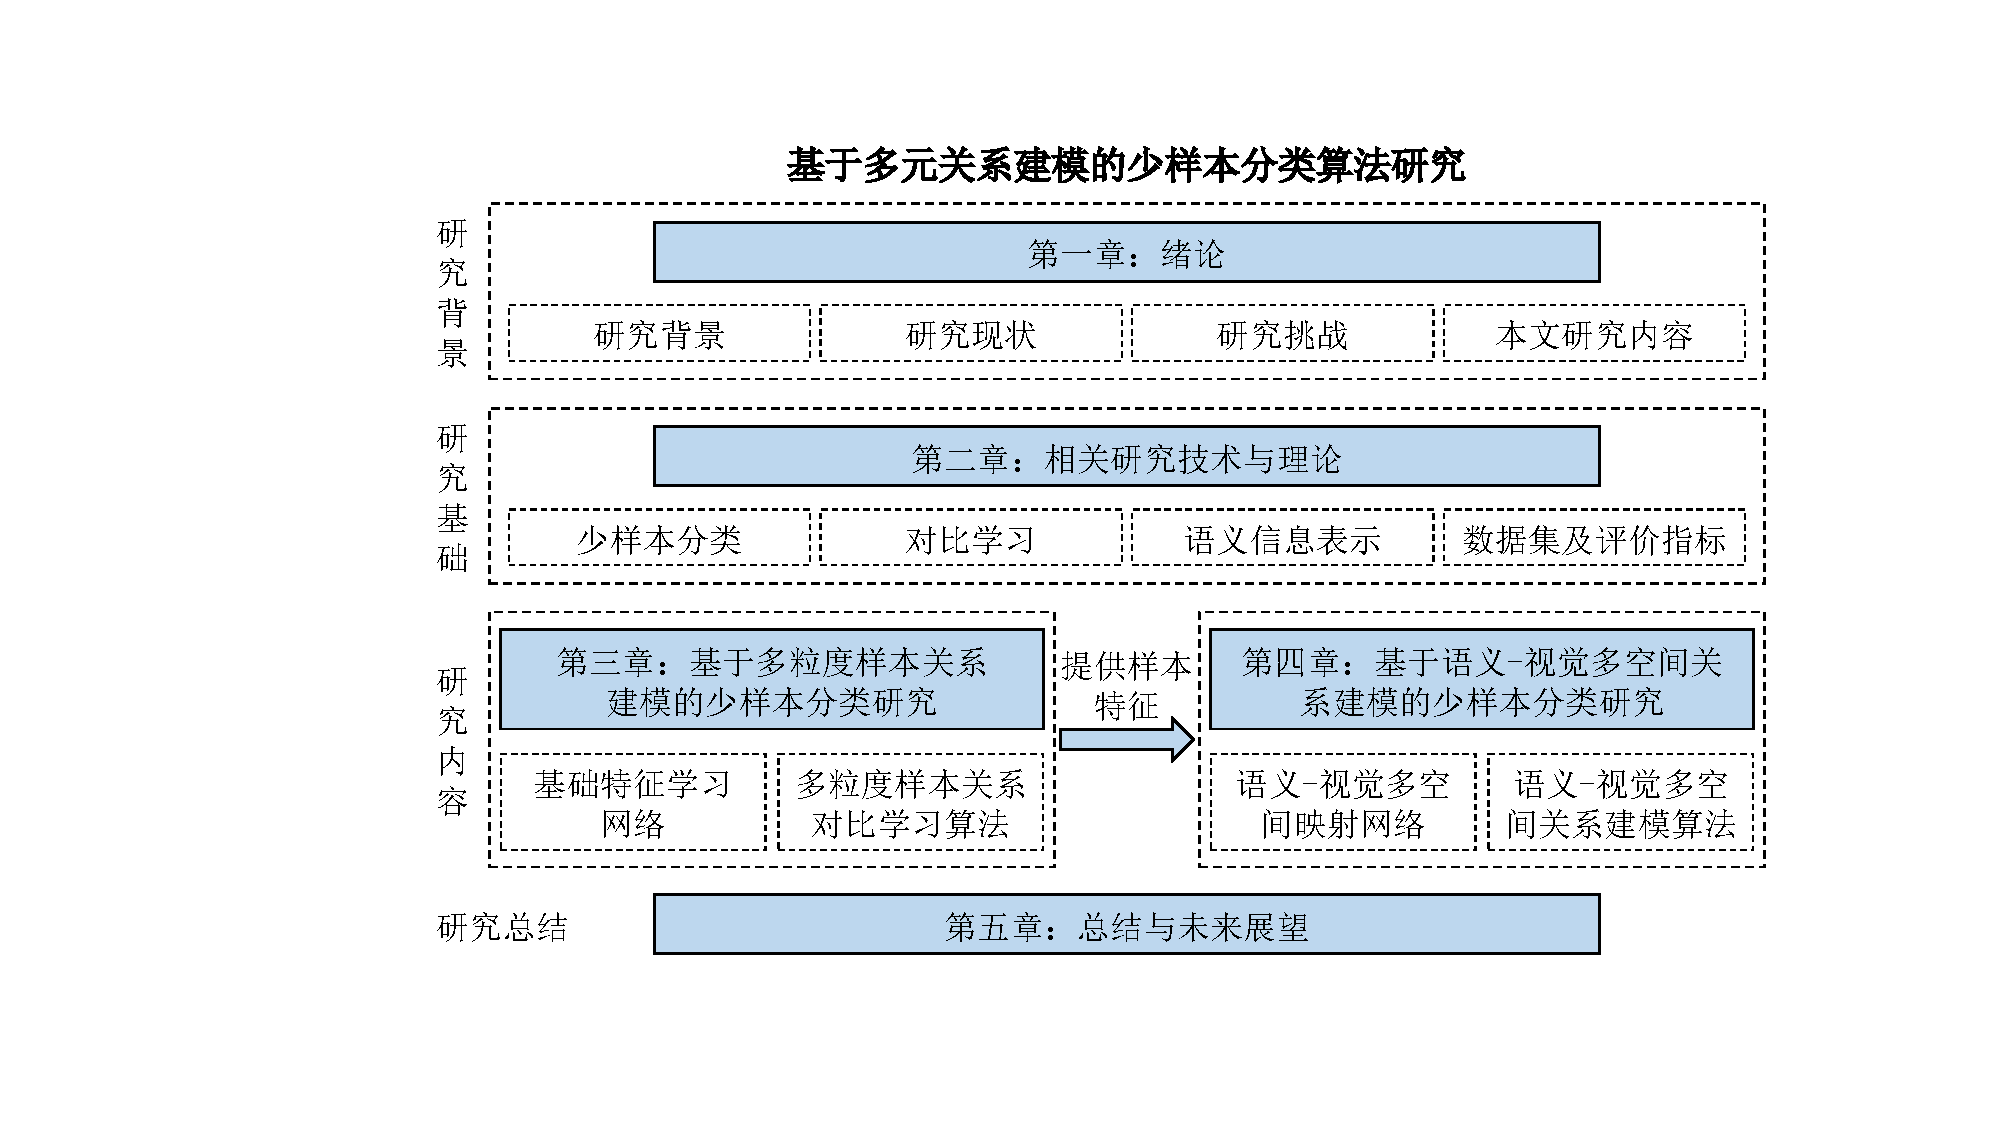
\includegraphics[width=1.0\columnwidth]{figures/组织结构.pdf}
%   \bicaption[本文组织结构图]{本文组织结构图。}[The organizational structure of the paper]{The organizational structure of the paper.}
%   \label{figure1: 组织结构}
% \end{figure}

% \section[\hspace{-2pt}本文组织结构]{{\heiti\zihao{-3} \hspace{-8pt}本文的组织结构}}\label{section1: 本文组织结构}

% 本文的组织结构图如图\ref{figure1: 组织结构}所示,共分为5个章节,各章节的介绍如下:

% 第一章:绪论。介绍少样本分类的研究背景和意义,并分析总结少样本分类算法的国内外研究现状及存在的挑战。最后对本文的研究内容和组织结构进行概述。

% 第二章:相关研究技术与理论。首先对少样本分类进行了进一步详细介绍,然后介绍本文方法中所使用到的对比学习技术以及语义信息表示,最后对本文实验所使用到的数据集及评价指标进行介绍。

% 第三章:基于多粒度样本关系建模的少样本分类研究。首先对部分现有少样本特征学习算法的不足进行分析,提出了基于多粒度样本关系对比学习的少样本特征学习算法(MGSRCL),随后详细介绍了针对不同粒度样本关系的建模方法,最后通过在四个基准数据集的大量实验证明了MGSRCL模型的有效性。

% 第四章:基于语义-视觉多空间关系建模的少样本分类研究。首先对基于语义的少样本分类算法进行分析介绍,提出了基于语义-视觉多空间关系建模的少样本特征适配算法(SVMSMA),然后介绍了SVMSMA模型的模型框架以及提出的跨模态分类和跨模态特征对齐模块,最后对所提方法进行了实验分析。

% 第五章:总结与未来展望。总结并分析了本文提出的基于多元关系建模的少样本分类算法研究的成果及不足,并对未来的研究方向与内容进行了展望。
